\chapter{Mathematical Identities}\label{app:math}

\section{Incremental Covariance Matrix Inverse}
% note the speedup expected
% In MATLAB backslash is optimized so speedup not observed.

The GP-update equations \eqref{gpUpdate_mu} and \eqref{gpUpdate_sigma}, require the inversion of the matrix $P_{t} \defeq K(x_{T}, x_{T}) + \sigma_{n}^{2}\mathbf{I}$. Since the CPG-UCB optimization \eqref{ucb} requires $\mu(x)$ and $\sigma(x)$ at each time step $t$, this matrix needs to be inverted at each step. The backlash operation to bypass this inversion requires $N^{3}/6$ complexity. For a single test point $x_{t}$, a workaround is to use incremental inverse for the growing matrix:

\begin{equation}
P_{t+1} = 
\left(
\begin{BMAT}(rc){c:c}{c:c}
P_{t} & k(x_{T}, x_{t}) \\
k(x_{T}, x_{t})^{\mathrm{T}} & k(x_{t}, x_{t})
\end{BMAT} 
\right)
\label{CovMat}
\end{equation}

where $k(x_{T}, x_{t}) \defeq (k(x_{1}, x_{t}), \ldots, k(x_{t-1}, x_{t	}))^{\mathrm{T}}$. 

The inverse of a general invertible $n \times n$ partitioned matrix 

\begin{equation*}
A = 
\left(
\begin{array}{cc}
P & Q \\
R & S \\
\end{array} 
\right)
\end{equation*}

is the $A^{-1}$ matrix:

\begin{equation*}
A^{-1} = 
\left(
\begin{array}{cc}
\tilde{P} & \tilde{Q} \\
\tilde{R} & \tilde{S} \\
\end{array} 
\right)
\end{equation*}

where the submatrices are given as \cite{GPbook}:

\begin{eqnarray}
\tilde{P} & = & P^{-1} + P^{-1}QMRP^{-1} \label{Phat}\\
\tilde{Q} & = & -P^{-1}QM \label{Qhat} \\
\tilde{R} & = & -MRP^{-1} \label{Rhat} \\
\tilde{S} & = & M \label{Shat}
\end{eqnarray}

and $M = (S - RP^{-1}Q)^{-1}$. Applying \eqref{Phat} - \eqref{Shat} on the inverse of the covariance matrix \eqref{CovMat} we get:

\begin{equation}
P_{t+1}^{-1} = 
\left(
\begin{BMAT}(rc){c:c}{c:c}
P_{t}^{-1} + \alpha P_{t}^{-1} q_{t} q_{t}^{\mathrm{T}} P_{t}^{-1}  & -\alpha P_{t}^{-1} q_{t} \\
-\alpha q_{t}^{\mathrm{T}} P_{t}^{-1} & \alpha
\end{BMAT} 
\right)
\label{CovMatInv}
\end{equation}

where 

\begin{eqnarray}
\alpha^{-1} & = & k(x_{t}, x_{t}) - q_{t}^{\mathrm{T}}P_{t}^{-1}q_{t} + \sigma_{n}^{2} \\
q_{t} & = & k(x_{t}, x_{T})
\end{eqnarray}

$\alpha$ is a scalar that is the outcome of the last point taken, $x_{t}$. \eqref{CovMatInv} can be reached easily by plugging the block matrices in \eqref{Phat} - \eqref{Shat} and noting that the covariance matrix $P_{t}$ is square symmetric.

A practical way to iteratively compute \eqref{CovMatInv} from $P_{t}^{-1}$ would be to compute first the vector of covariances $q_{t}$  and then $q_{t}^{\mathrm{T}}P_{t}^{-1}$, and apply it throughout the block matrices in \eqref{CovMatInv}. Figure \ref{fig:runtimes} shows the results for such an implementation in MATLAB running on Intel i7 1.6 GHz Quadcore laptop, where the runtimes for the matrix multiplication operation, $(K(x_{T}, x_{T}) + \sigma_{n}^{2}\mathbf{I})^{-1}\mathbf{k}_N(x^{*})$ is compared. The incremental matrix inversion is clearly faster, especially as the data sample size $N$ increases. Figure \ref{fig:deltaruntimes} shows the effect more clearly. Note that for the backslash method, the covariance matrix is not built from scratch at each iteration, but only the last row and column are added.

\begin{figure}
\center
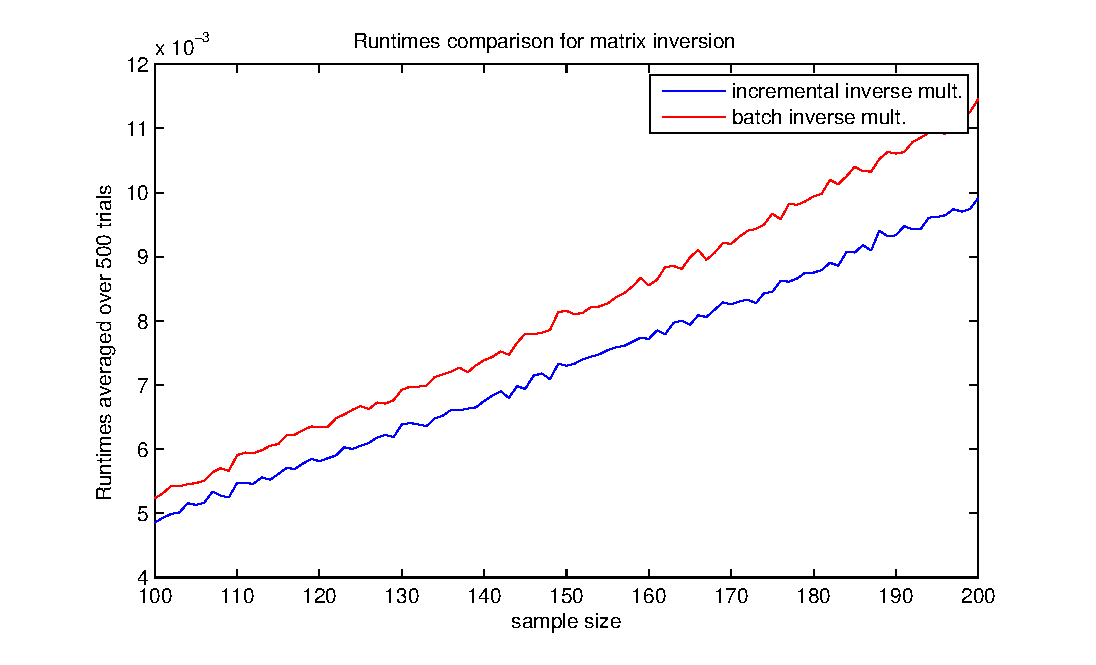
\includegraphics[scale=0.50]{runningtimes.eps}	
\caption{Runtime comparison}
\label{fig:runtimes}
\end{figure}

\begin{figure}
\center
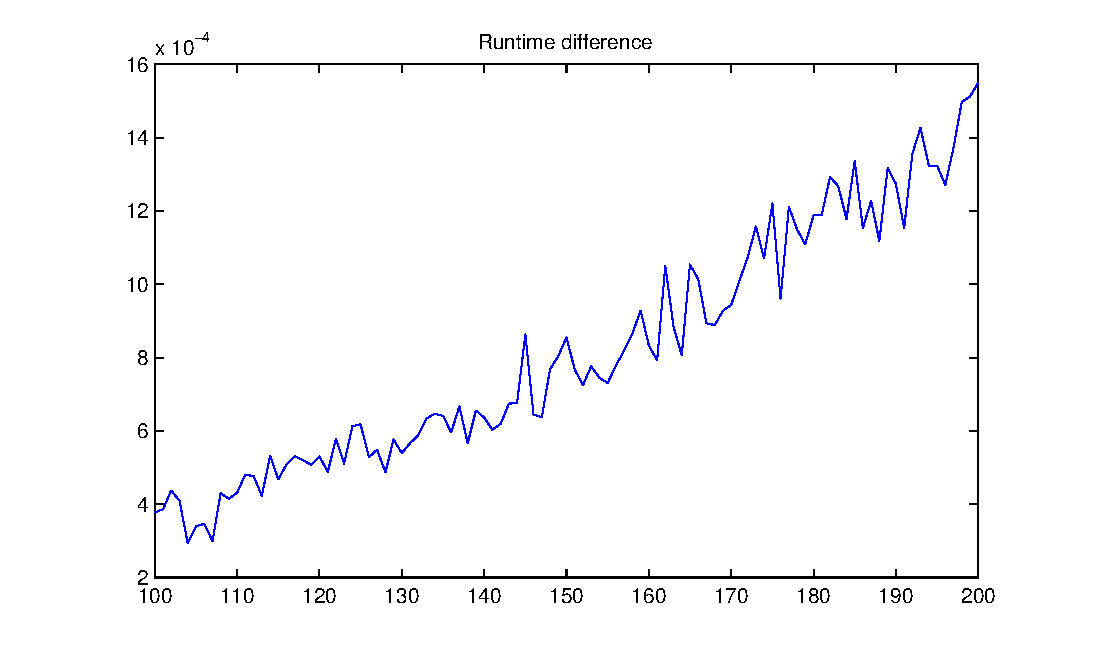
\includegraphics[scale=0.50]{delta_runningtimes.eps}	
\caption{Difference in runtimes}
\label{fig:deltaruntimes}
\end{figure}
